%!TEX root = thesis.tex
\chapter{Theoretical Concepts}\label{sec:chapter}


\section{Regression Problems}\label{sec:section}

\begingroup
Statistic models often contain many variables, which depend on each other.
Regression problems attempt to find this relationship by minimizing the expected
loss from a given model. $ N \in  \mathbb{N} $ samples are drawn from a set of samples
$ \{(\bm{x}_i, \bm{y}_i)\}^N_{i=1} $ using an unknown distribution $ P_{X,Y} $. A regression model
then computes a function that minimizes the loss
$ \mcl{L}(f(\bm{x}), \bm{y}) = \lvert\lvert f(\bm{x}) - \bm{y} \rvert\rvert^2_2 $. This loss is then
defined as the objective or cost function of the optimization problem.
\endgroup


\section{Neural Networks}\label{sec:section}


%%% Description of neural networks
\begingroup
Recent breakthroughs in text processing, image recognition and speech processing using DNNs
have led to significant performance increases \cite{GoogleTranslation, AlexNet, SpeechRecognition}. These biology inspired computational models generally rely on a feed forward architecture.
A set of inputs is propagated through the network to generate a certain output. The network itself is built using various nodes
or neurons. These neurons combine inputs of previous nodes to form an output tensor or vector. This operation is performed using a weight matrix.
This weight matrix $\bm{W}$ is usually optimized to minimize the output error for a classification or regression problem.

The processing of a single neuron as seen in \cite{Neural} uses a set of inputs, weights and biases to predict the output vector.
One of the simplest networks based on these assumptions is a perceptron, primarily used for binary classification tasks. The node
gets $\sum_{i=0}^{N}{w_i x_i + b_i}$ as an input and generates an output using an activation function $f$. Common
activation functions include the Binary Step, Sigmoid, Softmax, Tanh and Rectifier Linear Unit (ReLu). Generally, activation functions are chosen
based on the output space and input data of the network.

Some research like Goodfellow et al. \cite{Goodfellow} suggests that models are vulnerable to adversarial attacks due to their linear properties.
Adding nonlinear layers to the model like Gaussian processes (GP) should therefore significantly reduce the model's vulnerability.
Different papers have investigated this relationship through GP hybrid deep neural networks (GPDNNs).
Bradshaw et al. \cite{GPDNN} has shown that the classification error rate of adversarial examples can be significantly reduced by using a GPDNN.
\endgroup


\begin{figure}[h]

\centering
\begin{tikzpicture}
    \node[functions] (center) {$f$};
    % \node[below of=center,font=\scriptsize,text width=4em] {Activation function};

    % \draw[thick] (0.5em,0.5em) -- (0,0.5em) -- (0,-0.5em) -- (-0.5em,-0.5em);
    % \draw (0em,0.75em) -- (0em,-0.75em);
    % \draw (0.75em,0em) -- (-0.75em,0em);

    \node[right of=center] (right) {};
        \path[draw,->] (center) -- (right);

    \node[functions,left=3em of center] (left) {$\sum$};
        \path[draw,->] (left) -- (center);

    \node[weights,left=3em of left] (2) {$w_2$} -- (2) node[input,left=1cm of 2] (l2) {$x_2$};
        \path[draw,->] (l2) -- (2);
        \path[draw,->] (2) -- (left);
    \node[below of=2] (dots) {$\vdots$} -- (dots) node[left=1.4cm of dots] (ldots) {$\vdots$};
    \node[weights,below of=dots] (n) {$w_n$} -- (n) node[input,left=1cm of n] (ln) {$x_n$};
        \path[draw,->] (ln) -- (n);
        \path[draw,->] (n) -- (left);
    \node[weights,above of=2] (1) {$w_1$} -- (1) node[input,left=1cm of 1] (l1) {$x_1$};
        \path[draw,->] (l1) -- (1);
        \path[draw,->] (1) -- (left);
    \node[weights,above of=1] (0) {$w_0$} -- (0) node[input,left=1cm of 0] (l0) {$x_0$};
        \path[draw,->] (l0) -- (0);
        \path[draw,->] (0) -- (left);

		\node[input,above right=1.5em and 1.5em of left] (b) {$b$};
        \path[draw,->] (b) -- (left);
    % \node[below of=ln,font=\scriptsize] {inputs};
    % \node[below of=n,font=\scriptsize] {weights};
\end{tikzpicture}

\caption{Perceptron}

\end{figure}



% \begin{figure}[h]
% 	\centering
% 		\includegraphics[width=0.95\textwidth]{Ti_black.pdf}
% 	\caption{Hier eine Abbildung}
% 	\label{fig:image}
% \end{figure}


\section{Fully Connected Neural Networks}\label{sec:section}

\begingroup
Fully Connected Neural Networks (FCNNs) are the most basic neural network models. They
combine multiple perceptrons to form a distinct output. Training these networks is usually performed
through a process called backpropagation. In \autoref{fig:fcnnfigure} such a network is displayed.
The network is built using three main components: input layer, hidden layer and output layer. Hidden
layers can be stacked on top of each other to provide higher connectivity. In a FCNN
each node in a layer is connected to each node in the previous layer, as shown in \autoref{fig:fcnnfigure}.
\endgroup


\begin{figure}[h]

\centering
\begin{tikzpicture}[shorten >=1pt,->,draw=black!50, node distance=\layersep]
    \tikzstyle{every pin edge}=[<-,shorten <=1pt]
    \tikzstyle{neuron}=[circle,fill=black!25,minimum size=17pt,inner sep=0pt]
    \tikzstyle{input neuron}=[neuron, fill=green!50];
    \tikzstyle{output neuron}=[neuron, fill=red!50];
    \tikzstyle{hidden neuron}=[neuron, fill=blue!50];
    \tikzstyle{annot} = [text width=4em, text centered]

    % Draw the input layer nodes
    \foreach \name / \y in {1,...,4}
    % This is the same as writing \foreach \name / \y in {1/1,2/2,3/3,4/4}
        \node[input neuron, pin=left:$x^{(1)}_{\y}$] (I-\name) at (0,-\y) {};

    % Draw the hidden layer nodes
    \foreach \name / \y in {1,...,5}
        \path[yshift=0.5cm]
            node[hidden neuron] (H-\name) at (\layersep,-\y cm) {};

    % Draw the output layer node
    % \node[output neuron,pin={[pin edge={->}]right:Output}, right of=H-3] (O) {};

		\foreach \name / \y in {1,...,4}
				\node[output neuron, pin={[pin edge={->}]right:$x^{(L)}_\y$}] (O-\name) at (5 cm,-\y cm) {};

    % Connect every node in the input layer with every node in the
    % hidden layer.
    \foreach \source in {1,...,4}
        \foreach \dest in {1,...,5}
            \path (I-\source) edge (H-\dest);

    % Connect every node in the hidden layer with the output layer
    \foreach \source in {1,...,5}
				\foreach \dest in {1,...,4}
      			\path (H-\source) edge (O-\dest);

    % Annotate the layers
    \node[annot,above of=H-1, node distance=1cm] (hl) {Hidden layer};
    \node[annot,left of=hl] {Input layer};
    \node[annot,right of=hl] {Output layer};

\end{tikzpicture}

\caption{Fully Connected Neural Network}
\label{fig:fcnnfigure}

\end{figure}


\begingroup
However, before the network can provide any predictions, it has to be trained through backpropagation.
Backpropagation uses a cost function in the output layer to calculate the loss from the expected values to the predicted values
in the neural network. The cost function is usually defined as the quadratic loss shown in \ref{05_loss}. In this case $\bm{x}^{(L)}$
defines the last layer's output in the $L$-layered network. Alternatively, the output can be written as $f(\bm{x}^{(1)})$ where
$\bm{x}^{(1)}$ describes the input vector of the FCNN.

The DNN's loss can be minimized based on the weights and biases of the model. In the following,
$\forall l \in \{ 1, ..., L \}$ defines the number of layers and $n^{(l)} \in \mathbb{N}$ the number of nodes in a particular layer.
For example the number of neurons in the last layer is given by $N \triangleq n^{(L)}$. $\bm{y} \in \mathbb{R}^N$ defines the expected data based on a dataset or previous training.
To minimize the loss $\mcl{L} : \mathbb{R}^{N} \times \mathbb{R}^{N} \rightarrow \mathbb{R}$
\endgroup

\begin{equation}
\label{05_loss}
\begin{aligned}
  \mcl{L}(\bm{x}) = \sum_{j=1}^{N} \; (\bm{x}_j^{(L)} - \bm{y}_j)^2 = \lvert\lvert \bm{x}^{(L)} - \bm{y} \rvert\rvert^2_2
\end{aligned}
\end{equation}


\begingroup
a gradient descent approach is taken.
First of all, the derivatives to a given set of weights and biases is calculated through \ref{05_derivative_w} and \ref{05_derivative_b}.
In this context $\phi^{(l)} : \mathbb{R}^{n^{(l-1)}}\rightarrow \mathbb{R}^{n^{(l)}}$ describes the activation function,
$\bm{W}^{(l)} \in \mathbb{R}^{n^{(l)} \times n^{(l-1)}}$ the weight matrix, $\bm{b}^{(l)} \in \mathbb{R}^{n^{(l)}}$
the bias and $\bm{x}^{(l)} \in \mathbb{R}^{n^{(l)}}$ the output of the $l$-th layer.
Additionally, $\bm{z} \in \mathbb{R}^{n^{(l)}}$ is introduced to condense all equations. The index $j$ is the node number
in the current layer, while $i$ denotes the index of the previous one.
\endgroup


\begin{equation}
\label{05_z}
\begin{aligned}
  \bm{z}_j^{(l)} = \bm{b}_j^{(l)} + \bm{W}_j^{(l)} \bm{x}^{(l-1)}
\end{aligned}
\end{equation}

\begin{equation}
\label{05_x}
\begin{aligned}
  \bm{x}_j^{(l)} = \phi^{(l)}(\bm{z}_j^{(l)})
\end{aligned}
\end{equation}


\begin{equation}
\label{05_derivative_w}
\begin{aligned}
  \frac{\partial \mcl{L}}{\partial \bm{W}_{j i}^{(l)}} = \frac{\partial \bm{z}_j^{(l)}}{\partial \bm{W}_{j i}^{(l)}} \frac{\partial \bm{x}_j^{(l)}}{\partial \bm{z}_j^{(l)}} \frac{\partial \mcl{L}}{\partial \bm{x}_j^{(l)}}
\end{aligned}
\end{equation}


\begin{equation}
\label{05_derivative_b}
\begin{aligned}
  \frac{\partial \mcl{L}}{\partial \bm{b}_{j}^{(l)}} = \frac{\partial \bm{z}_j^{(l)}}{\partial \bm{b}_{j}^{(l)}} \frac{\partial \bm{x}_j^{(l)}}{\partial \bm{z}_j^{(l)}} \frac{\partial \mcl{L}}{\partial \bm{x}_j^{(l)}}
\end{aligned}
\end{equation}

\begingroup
After solving \ref{05_derivative_w} the negative gradient can be used to minimize the loss using a greedy method \ref{05_w}. The values for $\eta$
and $\gamma$ affect the convergence and learning speed of the model. If either one is too large the weights and biases will
oscillate around the optimal value. To avoid this problem the backpropagation algorithm can be further improved by applying smoothing and momentum strategies. These
strategies use a previous iteration step to filter out rapid changes in the cost function \cite{NeuralIntro, EffBackprop}.
\endgroup


\begin{equation}
\label{05_w}
\begin{aligned}
  \Delta \bm{W}_{j i}^{(l)} = - \eta \; \frac{\partial \mcl{L}}{\partial \bm{W}_{j i}^{(l)}}
\end{aligned}
\end{equation}

\begin{equation}
\label{05_b}
\begin{aligned}
  \Delta \bm{b}_{j}^{(l)} = - \gamma \; \frac{\partial \mcl{L}}{\partial \bm{b}_{j}^{(l)}}
\end{aligned}
\end{equation}

\begingroup
Models trained for adversarial testing during this thesis mainly rely on the Adam Optimizer. Adam, introduced by Kingma and Ba
\cite{Adam}, uses the stochastic gradient descent of the objective function. Rapid changes are filtered out using two exponential
moving averages, which define an update rule for the step size. The initial default step size is denoted by $\alpha$ and usually
has a value of around 0.001.
\endgroup


% Perturbation Analysis
\section{Perturbation Analysis}\label{sec:section}

\begingroup
The same intuition derived in the previous section can be a applied to a small perturbation of the input $\bm{x}^{(1)}$.
In signal processing a perturbation analysis or sensitivity analysis is used to quantify the output error with respect to a known perturbation at the system's input.
Efficient ways to calculate these output changes are especially important for the creation of adversarial examples.
The output of a layer for slight perturbations of $\bm{x}$ is given by
\endgroup

\begin{equation}
\label{05_phi}
\begin{aligned}
  \bm{\hat{x}}^{(l)} = \phi^{(l)} (\bm{W}^{(l)} \bm{\hat{x}}^{(l-1)} + \bm{b}^{(l)})
\end{aligned}
\end{equation}

\begingroup
To avoid gradient calculations for each layer \ref{05_phi} needs to be linearized. This is possible by applying
the first taylor expansion at the position $\bm{W}^{(l)} \bm{x}^{(l-1)} + \bm{b}^{(l)}$.
\endgroup

\begin{equation}
\label{05_error}
\begin{aligned}
  \bm{\hat{x}}^{(l)} &= \phi^{(l)} (\bm{W}^{(l)} \bm{\hat{x}}^{(l-1)} + \bm{b}^{(l)}) \\
   &= \phi^{(l)} (\bm{W}^{(l)} (\bm{x}^{(l-1)} + \Delta \bm{x}^{(l-1)} ) + \bm{b}^{(l)}) \\
   &\approx \bm{x}^{(l)} + \bm{J}_{\phi^{(l)}} (\bm{W}^{(l)} \bm{x}^{(l-1)} + \bm{b}^{(l)}) \bm{W}^{(l)} \Delta \bm{x}^{(l-1)}
\end{aligned}
\end{equation}

\begingroup
This enables consecutive multiplication of the output error for each layer. This is
usually done by diagonalizing $\phi^{(l)}$ according to \cite{NeuralError}.
\endgroup

\begin{equation}
\label{05_diagonal}
\begin{aligned}
  \bm{D}^{(l)} = diag( \phi^{(l)'} (\bm{W}^{(l)} \bm{x}^{(l-1)} + \bm{b}^{(l)}) )
\end{aligned}
\end{equation}

\begingroup
Afterwards the perturbation of $\Delta \bm{x}^{(l)}$ in relation to $\bm{x}^{(l-1)}$ is
described by
\endgroup

\begin{equation}
\label{05_output}
\begin{aligned}
  \Delta \bm{x}^{(l)} = (\bm{D}^{(l)} \cdot \bm{W}^{(l)}) \; \Delta \bm{x}^{(l-1)}
\end{aligned}
\end{equation}

\begingroup
Applying this technique to all the layers in the neural network then leads to \ref{05_largez}
and \ref{05_finish}.
\endgroup

\begin{equation}
\label{05_largez}
\begin{aligned}
  \bm{Z}^{(l)} = \prod_{i=1}^{l} \bm{D}^{(i)} \cdot \bm{W}^{(i)}
\end{aligned}
\end{equation}

\begin{equation}
\label{05_finish}
\begin{aligned}
  \Delta \bm{x}^{(l)} \approx \bm{Z}^{(l)} \; \Delta \bm{x}^{(0)}
\end{aligned}
\end{equation}

\section{Convolutional Neural Networks}\label{sec:section}

\begingroup
Unfortunately, FCNNs do not scale well for images. Even using smaller image datasets like MNIST (28x28x1) or CIFAR (32x32x3)
leads to a large amount of weights with multiple hidden layers. This becomes even more problematic for larger images.
Additionally, the large amount of parameters may lead to overfitting in the network according to the provided input data.
In this section Convolutional Neural Networks (CNNs) are discussed as an alternative solution.
One of the earliest advances in CNNs were based on character recognition by LeCun et al. \cite{LeCun}. Nowadays, these networks
are used for a variety of image classification tasks. For instance, Krizhevsky et al. \cite{AlexNet} was able to beat
state-of-the-art classification techniques for the ImageNet challenge using a CNN. The structure of a CNN resembles ordinary
NNs. CNNs are also built using trainable weights and biases. Neurons in the network receive an input vector
and perform a dot product on the trained weights. Optionally, an activation function is then applied to the result.
Therefore, general concepts developed in the previous section still apply.

In contrast to a regular FCNN, CNNs are specifically designed to receive images as an input.
This significantly reduces the amount of parameters in the network and therefore also improves the overall efficiency.
To achieve this, the CNN architecture arranges neurons in 3 dimensions (i.e. 32x32x3 for the CIFAR-10 input volume).
Neurons in each layer are only connected to a small area of the previous layer. Usually the volume decreases with an
increasing number of layers. For instance, classification tasks of the CIFAR-10 dataset would lead to an output volume of
1x1x10.

The architecture is built using three different layer types. These layers are convolutional layers, pooling layers
and fully-connected layers. The structure usually resembles \autoref{fig:cnn}. First a convolutional layer applies different
filters to the input image channels. Then a pooling layer reduces the volume size. At last, a fully-connected
layer is used to generate an arbitrary output volume (e.g. classification classes).
\endgroup

\begin{figure}[ht]
\centering
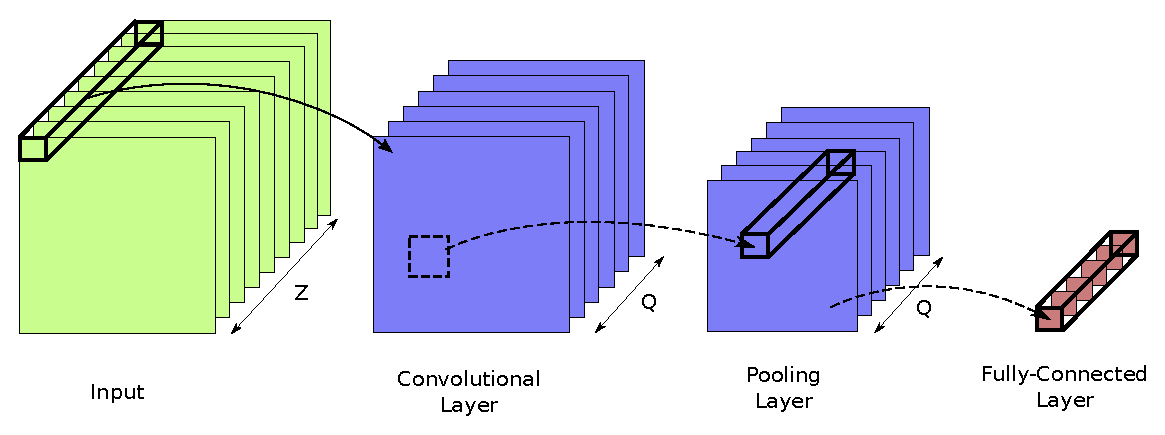
\includegraphics[width=.7\linewidth]{deep.eps}
\caption{Convolutional Neural Network Structure}
\label{fig:cnn}
\end{figure}


\begingroup
The convolutional layer uses different filters and computes the dot product between a small region in the previous layer and a set of weights. The output
of this calculation is usually described as an activation map. The computation for a single input layer and filter is shown in \autoref{fig:convlayer}.
The output for this filter is calculated through $1*1 + 1*1 = 2$. For multiple convolutional layers the activation maps are stacked on top of each other.
The number of filters is specified by $Q$ in \autoref{fig:cnn}. The input depth is defined by $Z$.
To control the output size of a convolutional layer depth, stride $S$ and zero-padding $P$ are used. Depth describes
the number of filters, which separately learn a different feature set. Stride specifies the number
of pixels a filter is moved. Zero-padding defines the padding used on the edges of input image. It is usually used to generate a
specific output. The output size of a convolutional layer is given by $(W - F + 2P)/S + 1$, where $W$ is the input
size and $F$ the filter size. If $S = 1$ zero-padding can be set to $P = (F - 1)/2$ to retain the input dimensions. Although this approach is only
presented for quadratic layers, $W$ and $F$ can be separately defined for each dimension.
\endgroup


\begin{figure}[ht]
\centering
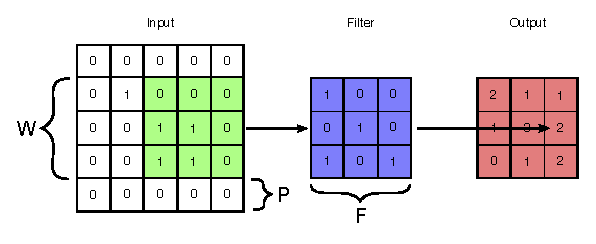
\includegraphics[width=.7\linewidth]{conv.eps}
\caption{Convolutional Layer Computation}
\label{fig:convlayer}
\end{figure}


\begingroup
Since convolutional layers usually add a lot of neurons to the model a pooling layer is applied to reduce the number of nodes.
The most common pooling layer simply finds the maximum value within a specified window and passes it on to the next layer.
This leads to a downsampling of the information in the current layer. Additonal fully-connected layers can be used to generate
a specific output volume \cite{ConvGit, ConvIntro, ConvVisual}.
\endgroup


\section{Autoencoders}\label{sec:section}

\begingroup
Autoencoders (AEs) are artificial neural networks used for efficient data encodings. These codes are found by creating
NNs that reproduce some input at the network's output. The structure of such a network is shown in \autoref{fig:autoencoder}.
The autoencoder is built using an encoding and decoding unit. The encoding unit compresses the input layer into
a lower-dimensional representation. The decoder of the autoencoder then uncompresses this code into a set of attributes
that closely matches the original input. This approach enables the network to ignore noisy input data. Another
advantage of autoencoders are non-existent data errors, since output and input are equivalent. Using other datasets might
introduce training errors into the model. In contrast, identity functions are easily verifiable.

After an autoencoder is trained each output usually has a unique latent representation in the network. This representation is
labelled as "Code" in \autoref{fig:autoencoder}. Apart from its compression characteristics, this code is used in
variational autoencoders (VAEs) to generate an output from a set of randomly chosen features \cite{VariationalAutoencoders}.
Furthermore, autoencoders can also be used to colorize and create higher resolution images. Both types
of autencoders are tested against adversarial attacks in this thesis.
\endgroup


\begin{figure}[ht]
\centering
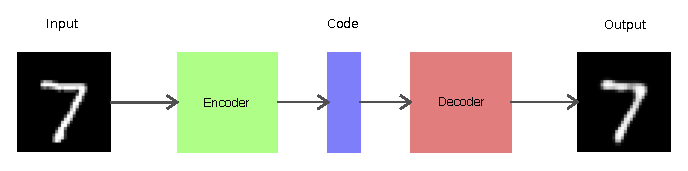
\includegraphics[width=.7\linewidth]{autoencoder.eps}
\caption{Autoencoder}
\label{fig:autoencoder}
\end{figure}

\begingroup
Instead of limiting the capacity of the network through its layers. It is possible to promote certain sets of features
through regularized autoencoders. For instance, sparse autoencoders are typically used to learn features for another
task such as classification. An autoencoder that has been regularized to be sparse must respond to unique features of
a dataset instead of acting as an identity function. Another class of regularized autoencoders are denoising autoencoders.
These networks attempt to remove noise that is added to an input image \cite{Denoise}.
\endgroup
